
\documentclass[11pt]{amsart}
\usepackage{geometry} % see geometry.pdf on how to lay out the page. There's lots.
\geometry{a4paper} % or letter or a5paper or ... etc
% \geometry{landscape} % rotated page geometry
\usepackage{url}
\usepackage{graphicx}
\graphicspath{ {images/} }
% See the ``Article customise'' template for come common customisations

\title{Peer to Peer Vs Client-Server : Which is Better?}
\author{
Peter Keogh
\\DT228C
\\Advanced Software Development
\\D94140029
}
\date{}

%%% BEGIN DOCUMENT
\begin{document}

\maketitle
%%%\tableofcontents

\section{Introduction}

Ubiquitous Computing can be defined as computation, communication and sensing being integrated with the physical world. First described in the paper by Mark Weiser ``The Computer in the 21st Century'', it is a paradigm where computers would ``disappear. They (would) weave themselves into the fabric of everyday life until they are indistinguishable from it.''\cite{Weiser} The pervasiveness of computers is the defining characteristic of Ubicomp, as a result it's applications touch on and integrate a broad range of topics within computer science and electronic engineering. Ubicomp has the potential be utilised in any and every industry or part of life. 
\paragraph{}

The choice of network architecture in the design of a ubiquitous computing system is crucial to the success of the system. The number of devices owned by a single user and has increased the amount of data produced and exchanged by systems. This has brought with it an increased load on networks exchanging this data. As ubicomp systems become more and more common this load is set to increase. Therefore determining how data will be exchanged and stored in a systems architecture is crucial to the success of Ubicomp. 
\paragraph{}

With such a broad range of devices and potential applications it is impossible to truly say that one network architecture is better than another. Client-Server networking and Peer-to-Peer networking both have their strengths and weaknesses. We cannot look at one and say that it is better that the other. We can however look at them and determine which is better for a particular application. This paper will present information that will hopefully help guide the decision making process when developing an application.

\paragraph{}
The growth of the internet has seen the emergence of two typical network architectures in many applications. These architectures are the Client-Server model and the Peer-to-Peer model. 
\paragraph{}
The popularity of these architectures can be easily seen when we look at their respective shares of network traffic. Although in recent years video over IP has come to dominate internet traffic we can still get a sense of the popularity of these architectures.  
Fixed web and data, mostly client-server services currently account for 5,625 Petabytes of data transfer a month. Similarly P2P file transfer consumes 5,254 Petabyes of data worldwide per month.\cite{Cisco}

Both P2P and Client-Server are not restricted to being independent of one another. In fact, companies such as Spotify and Skype use a hybrid approach.
%I believe we will see a further blurring of the lines between client server and p2p.

\section{The Architectures}

\includegraphics[scale=.5]{Architectures}

\subsection{Client-Server}

\paragraph{}
Many of the most successful technology businesses are based on the Client-Server model today, most obviously in Cloud Computing. Gmail, Facebook and Dropbox are all examples of applications built on the client-server architecture. It is an appealing architecture for these businesses as they can store and access customer information. The advent of faster and more reliable internet access in many parts of the world and the growth in the number of connected devices users have also contributed to the growing popularity of this architecture. 
\paragraph{}
People want to be able to access their resources on all of their devices. Client-server architectures make this possible. In years gone by users would have to back all their work up on a CD or floppy disk. They would forget to do so at their peril. Now one can work on a project locally and easily save it to a remote server to back it up. 
\paragraph{}
Using cloud services is appealing to users as it can allow the user to spend less money on their devices. ``Thin'' clients like Google's Chrome book have come to fill a new gap in the market. As services such as Google Docs provide a cloud alternative to Microsoft Word the processing and storage requirements of a laptop can be minimised.

%	This is very much from the book - Computer networking, a top down approach and needs to be fleshed out with other sources.
%	I also need to phrase all of this better in my own words
\paragraph{}
In the Client-Server Architecture one always-on host known as a server services requests from other hosts known as clients. The clients exchange data with the server and the server provides the clients with services. 
\paragraph{}
The classic example of a client server architecture is in web applications. A client, usually a web browser sends a request to the server using the http protocol. The server then responds by sending a html page for the browser to render. In a client-server application clients do not directly communicate with each other. They can communicate with each other via the server. For example, in the Facebook chat application a client can send a message to the server using AJAX which the server forwards to another client. To the user it appears the same as if the two clients were communicating directly. The server has a fixed IP address which is known or can be discovered by any client that wishes to connect to it.
\paragraph{}
Increasing numbers of clients typically put more strain on a server. As one host needs to accommodate many requests it requires a robust infrastructure. Usually a single host isn't enough and more complex distributed application architectures need to be developed. These architectures typically make use of server farms; large warehouses filled with servers that are capable of communicating.

\subsection{Peer-to-Peer}
\paragraph{}
P2P first emerged in the popular conscious in the form of Napster. It has caused quite a stir in the past and continues to do so. It's most common use is file sharing, often illegally. It's use in this manner has had a major impact on the entertainment industry and as a result they have lobbied continuously for it's regulation.
\paragraph{}
 P2P offers advantages over the client server model. In the case of file sharing P2P provides a greater availability of popular material. The more popular a resource is the more likely a peer is to be sharing it. As a result it can be more robust than a client server model, in which, once the server goes down the client is unable to avail of it's resources. On the other hand, if a resource is unpopular it is unlikely that many peers will be seeding that resource at any point in time. In this case a client server architecture might be preferable.
\paragraph{}
In the Peer-to-Peer (P2P) Architecture nodes communicate directly and intermittently. The hosts in a P2P architecture are known as peers. Reliance on always on servers tends to depend on the ``purity'' of the P2P application. An application with no reliance on servers could be said to be ``pure'' P2P. P2P provides many opportunities the development of applications that require collaboration, decentralisation or high network throughput. This has lead to it's use in popular applications such as BitTorrent and BitCoin.
\paragraph{}
A P2P architecture is 'self-scalable'. While the addition of an extra peer increases the workload of the system by increasing the number of requests the peer also increases the ability to handle that workload by providing the service to other peers. Securing P2P applications can be difficult due to their open and distributed nature.
\paragraph{}
P2P can be broken down further into three subcategories of architecture; centralised, decentralised and hybrid P2P.
\paragraph{}
An example of centralised P2P would be BitTorrent. In order to communicate with peers in the network a client must obtain information about the peers from a centralised server known as a tracker. Information about a tracker is obtained from a metadata file. A user needs to visit centralised server such as The Pirate Bay or Kick Ass Torrents in order to obtain this file. This dependence on a centralised server to track the network is what defines BitTorrent as centralised P2P.
\paragraph{}
In a decentralised or pure P2P Architecture each peer acts as an indexed server. It also acts like a router by relaying queries between peers. An example of this would be BitCoin or Gnutella 0.4.
\paragraph{}
In hybrid P2P hosts with a good internet connection act as routers for other peers in the network who's connection isn't as strong. An example of this is Gnutella 0.6.

%ELABORATE HERE 
\paragraph{}
Peer-to-peer systems are most effective at storing large amounts of immutable data. They perform less well at storing mutable data.\cite{DistSys}
%%% from distributed computing book

%%% Look at this: http://medianet.kent.edu/surveys/IAD06S-P2PArchitectures-chibuike/P2P%20App.%20Survey%20Paper.htm
\section{Example Protocols}

A protocol is an agreed method of communicating between applications. The protocols outlined below provide details of how current technologies using the architectures outlined above communicate. While these particular protocols may not be directly applicable to Ubicomp directly they provide a useful outline of how the architectures need to work in reality. Designers of Ubicomp systems are likely to encounter similar problems that system designers have encountered in the past. These protocols outline methods for overcoming these problems. An outline of these protocols will be useful in reasoning about the architectures as applied to Ubicomp systems later.

\subsection{HTTP Protocol}
\paragraph{}
The client-server architecture is the typical architecture used in web applications. The protocol used for transferring information between the client and server is the HTTP protocol. HTTP (HyperText Transfer Protocol) follows a request response cycle. The client makes requests to the server and the server responds to the request. The server doesn't send any information to the client if not prompted by a request. This has implications for applications using the protocol. 
\paragraph{}
If nodes wish to collaborate with each other or obtain realtime information about other nodes in the system they must ``poll'' the server by repeatedly sending requests to the sever. This is very inefficient as it results in significant network overhead and results in the server processing requests even when the state of the system remains unchanged. A solution for this problem has recently emerge the the standard of web sockets which allows servers and web browsers to set up a dedicated end to end bidirectional connection.
\paragraph{}
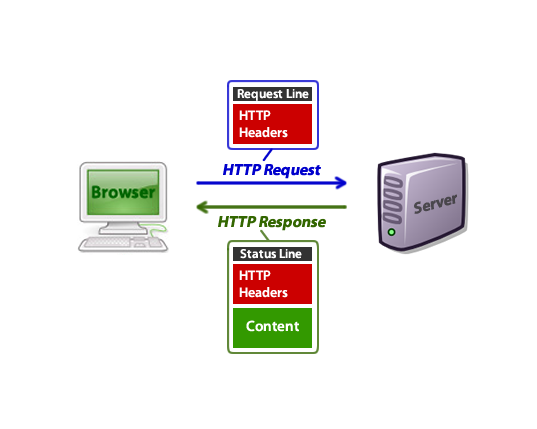
\includegraphics[scale=.7]{http_diagram}\cite{http://probablycopyrighted.com/wp-content/uploads/http_diagram.png}

\subsection{Gnutella 0.4}\cite{GnutellaCase}
\paragraph{}
Gnutella was the first large scale decentralised P2P network of it's kind. It ``builds at the application layer a virtual routing mechanism.''\cite{GnutellaCase} Early versions of Gnutella were truly decentralised P2P networks. No centralised servers were needed to facilitate the transfer of files from node to node.
One of the implications of not using centralised servers in a p2p application is the challenge of keeping track of network nodes and what resources are available in the network. In order to obtain this information ``network flooding'' was used. Peers all maintain at least one TCP connection to other nodes in the system. The network flooding algorithm ``floods'' the network with requests; each node sends messages on to all of it's neighbours except the one it received the message from. 
\paragraph{}
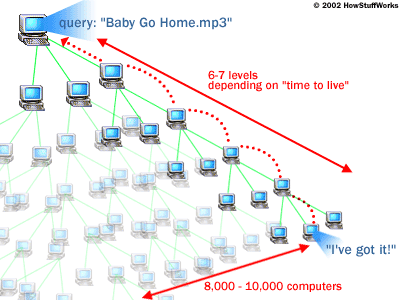
\includegraphics[scale=.9]{file-sharing1}\cite{http://static.howstuffworks.com/gif/file-sharing1.gif}

\subsection{Gnutella 0.6}\cite{GnutellaCase}
\paragraph{}
The flooding model used in Gnutella 0.4 had scalability problems. Searches were costly and usually terminated prematurely. Gnutella moved from a ``pure'' P2P paradigm to a hybrid approach. This new approach makes use of ultra peers and leaf nodes to create a hierarchically structured network. An ultra peer is a node that has a faster connection and elects to route more traffic for the network. The ultra peers also act as proxies for the leaf nodes. Searches become more efficient since searches only need to flood the ultra nodes instead of the whole network.


\subsection{Bittorrent Protocol}\cite{Bittorrent} \cite{BittorrentSpec}
\paragraph{}
The bit torrent protocol is a P2P file sharing protocol that runs over HTTP and TCP. The owner of a file hosts a ``bencoded'' metadata file (with the extension .torrent) on a server. A user downloads the metadata file and opens it in a bit torrent client. This client uses a url contained in the metadata file to connect to a ``tracker''. A tracker is a HTTP service that maintains information about the torrent, including a list of peers. The tracker may also provide stats for the torrent at a``scrape'' url.
\paragraph{}

Once a client has obtained information from the tracker it can communicate with peers using TCP. Peers exchange the blocks defined in the metainfo file. Peers all have connections with each other that they maintain state info about. Peers exchange information based on these states.
\paragraph{}
These states are choked and interested. A peer may choke a client to stop it requesting data. A peer is interested if the client has something that the peer wants. If a peer is interested it can unchoke the client so they can begin exchanging data.

\section{Comparison of Performance}

Systems that are built with the Client-Server architecture and P2P systems are both examples of distributed systems. There are several challenges associated with distributed systems that provide interesting metrics to analyse these architectures under. These are:

\begin{itemize}
  \item Performance, the amount of work a system can do. 
  \item Scalability, the ability of the system to handle greater loads and to get bigger. 
  \item Security, the ability to keep malicious parties from doing things to or with our system we don't want them to do.
\end{itemize}

\subsection{Availability, Fault Tolerance and Scalability}

\paragraph{}

Availability in client-server systems is dependent on the server architecture and network connection. If a firewall is preventing a user from accessing a server then to that user the server is unavailable.

\paragraph{}
A single server may be enough to handle requests for a service with few customers making infrequent requests. In the case of a sever simply providing static information for clients a single server can usually handle all the requests that are made of it. However, more popular and complicated services that require more processing and data throughput need more complicated server architectures.

\paragraph{}
 A service that works internationally can reduce the network latency of requests in certain regions by having the same service running on multiple servers in locations that are closer to their customers. This reduces the load on a single server and has the added advantage that we can partition customer's data to be located closer to them.

\paragraph{}
Data can be managed through replication and partitioning. Data can be partitioned so that data that are frequently accessed together can be stored together. By replicating data the system becomes more fault tolerant; if one server crashes the data can be accessed at another.

\paragraph{}
All of the techniques for improving availability, fault tolerance and scalability in client-server architectures come at a cost. There's the financial cost of paying for more storage and processing power. There's also cost associated with developer time. Developing and deploying distributed server architectures can be time consuming and expensive not to mention complicated. While replicating data improves the fault tolerance of the system they system now needs to make sure that the data is consistent throughout the system. There is also an additional cost associated with system administration.\cite{DistSys}

\paragraph{}
\paragraph{}
Availability in P2P systems is a function of the number of system nodes and the popularity of the resource to be accessed. If a node wishes to request a resource that is popular in a network with a large number of nodes then it should have no problem getting it. It is likely that there will be nodes geographically nearby that are hosting the information and are currently available for processing. This would result in reduced network latency and a faster download of the resource.

\paragraph{}
For example, if a BitTorrent user wanted to download Miley Cyrus's ``Bangerz'' album they would find 1143 peers hosting that file according to The Pirate Bay. That resource would be highly available in the P2P system.\cite{Miley}

\paragraph{}
If on the other hand a user wanted to read ``Everyware, The Dawning Age of Ubiquitous Computing'' they would find just 3 peers hosting the file. This file would be far less available than Cyrus's album. A user attempting to download this album would only be able to download the resource when at least one peer was active.\cite{Everyware}

\paragraph{}
If a user wanted to obtain a copy of the academic paper ``Supporting Activity in Desktop and Ubiquitous Computing''. It is unlikely that there would be a peer actively hosting this file. A Pirate Bay search revealed no results for this resource at this time.
This illustrates just one problem of availability in P2P networks. Niche resources like academic journals are better hosted on a server. Real world institutions can't function based on what's popular. 

\paragraph{}
One important thing to note is that when a user downloads ``Everyware, The Dawning Age of Ubiquitous Computing'' they increase the availability of the resource. If they choose to host the files then there would be 4 peers for the next user to download from. The availability of a resource increases in proportion to the nodes in the system with that resource.

\paragraph{}
P2P is also extremely fault tolerant if the network is big enough. If a cup of coffee spills over one of the nodes in the Miley Cyrus network the downloading peers are unlikely to notice a performance difference.
P2P is at it's most fault tolerant when it is completely decentralised and has no reliance on centralised trackers.

\paragraph{}
P2P networks are highly scalable as a result of all of the above since an increase in the number of clients consuming network resources increases the ability of the network to handle it's load. 

\subsection{Security}
\paragraph{}
All software systems that are networked have similar vulnerabilities. The network connection can be eavesdropped on. Data stored can be accessed without permission. It is considered good practice to encrypt any sensitive data that is transferred or stored.
\paragraph{}
One of the most common attacks on a server is a denial of service attack. An attacker floods a resource with requests to make the resource unavailable for others.\cite{DistSys} One of the advantages of Client Server architectures is that once a security risk is identified it can be fixed for the whole system by a system administrator. This is in contrast to P2P where software must be updated on a huge number of machines by a huge number of owners.
\paragraph{}
One of the main methods of attacking a peer-to-peer network is to have multiple nodes conspiring against the other nodes in the system. In the case of bit coin the only way to achieve this is to have more that half of the nodes behaving maliciously.\cite{bitcoin} In order to make this happen the attacker would need access to a number of hosts beyond the budget of any hacker. One strategy for attacking a P2P network using conspiring nodes is to provide false information to other nodes in the network.
\paragraph{}
An obvious security issue in P2P systems is the code to be run has access to the filesystem of a user. In the case of systems that share files like BitTorrent users need to know that they can trust the code of the torrent client they use. In a more complicated p2p system where users could contribute arbitrary code there would need to be mechanisms in place to protect the system from this code.

\section{Social and Political Issues}

There are a number of important political and social issues surrounding the choice of architecture for a particular application.

\subsection{Jurisdiction}
\paragraph{}
The client server model has brought with it legislative challenges for governments. European data protection authorities have had trouble enforcing local legislation with companies based abroad. Multinational companies such as Google tend to argue that since they are based in California then EU Data Protection laws don't apply to them. Others argue that the physical location of data determines which jurisdiction it resides in. 
\paragraph{}
Even if this is the case, companies may have to obey the laws of their home country if they control the data regardless of the location of the data. Data stored on European servers by an American company may be given to the United States Government under the Patriot Act. Both Amazon and Microsoft have said they would give the US Government access to their European cloud under the Patriot Act.\cite{Forbes}

\subsection{Censorship}
\paragraph{}
The client server model used in traditional web applications is far easier for governments to censor than peers to peer networks. Governments can force internet service providers to block IP addresses, redirect domain name requests to bad IP addresses or force a hosting company to remove a service from it's servers. This is the case in countries like China where the government's ``Great Firewall'' prevents Chinese netizens from accessing sites like Facebook, Google and Twitter. These services have come to be replaced by Chinese equivalents like Baidu, Renren and Sina Weibo. These sites are subject to heavy regulation from the Chinese government. 
\paragraph{}
In Ireland there is a certain amount of internet censorship. Eircom has been ordered to block sites associated with illegal file sharing such as The Pirate Bay.
\paragraph{}
The centralised nature of the client server model makes it easy for governments to censor applications built on it. One of the reasons for this is because it is easy to shutdown a system with a single point of failure.
\paragraph{}
One of the methods of bypassing such censorship is by leveraging the P2P model. In January 2014 The Pirate Bay announced that it was developing ``a browser-like client to circumvent censorship, including domain blocking, domain confiscation, IP-blocking.'' The software works like both a web browser and a BitTorrent client. Web application files that would usually be stored on a centralised server are instead shared among peers. The application has it's own DNS system in which it uses a fake DNS that links to a unique and verified public key.\cite{PirateBayBrowser}
\paragraph{}
Another example of a project that utilises the P2P model to bypass web censorship is the Freeweb project conceived by Shen, Liu and Zhao.\cite{FreeWeb} This model functions differently to the Pirate Bay system. In Freeweb nodes in regions not subject to censorship act as proxies for nodes in regions that are. 



\subsection{Privacy, Spying and Hacking}
\paragraph{}
Services such as Facebook and Google offer ways of communicating and discovering information that they collect in their servers. While most people consider these services free they do come at a price. It's an internet cliche now that ``If You're Not Paying for It; You're the Product.'' In light of the revelations revealed by Wikileaks and whistleblowers like Edward Snowden the public have started asking if the convenience of these services is worth trading their privacy for.
\paragraph{}
Client server technologies offer us the opportunity to automatically back up data to a cloud account. Services like Apple's iCloud allow users to synch their iPhone data automatically. Many users simply set this up and don't think about it again until something goes wrong with their device. Users may be unaware of what they are synching. Having so much personal data automatically synched to a cloud service provides a gold mine for hackers. Recently many hackers have released personal photos of celebrities such as Jennifer Lawrence that were synched to iCloud.

\subsection{Copyright and Free Riding}
\paragraph{}
P2P networks such as bit torrent have been notoriously used for illegal file sharing since Napster. Attempts were made to crack down on this file sharing in legislation such as the Stop Online Piracy Act (SOPA). SOPA was eventually abandoned after websites such as Reddit and Wikipedia protested the legislation with a blackout day. The size of P2P networks and the amount of file sharing that happens within them makes it extremely difficult and expensive to prosecute.
\paragraph{}
One of the issues in P2P networks is the social dilemma of ``free riding''. In a file sharing system the availability of a resource is dependent on peers sharing that resource. However, if peers choose not to share the resource they can improve their network bandwidth and download more resources for themselves. A consequence of this is that as fewer and fewer peers are sharing it becomes easier to prosecute file sharers. \cite{FreeRiding}


%\subsection{Net Neutrality}

\section{Notable Systems and The Architectures in the Context of Ubiquitous Computing}
\paragraph{}
It's easy to compare P2P and the client-server model as they are being currently utilised. While it is tempting to believe these models to be analogous to these architectures in Ubiquitous computing, that is not necessarily the case. The requirements of a Ubiquitous Computing system are different from systems that have been used in the past. For example, ubiquitous computing systems are likely to produce large amounts of data as a result of the numbers of sensors in the systems. Storing all of this data on server would probably be overkill not to mention expensive.
\paragraph{}
The choice of network architecture impacts the development of technology. A prime example of this is in the development of the World Wide Web. Web browsers are no longer simple programs that display HTML. One of the motivations for this has been to reduce the load on servers. Why should a server waste precious processing power assembling HTML views that can be created on the fly by a browser.
\paragraph{}
This can be contrasted with Wireless Sensor Networks. Currently sensors, particularly on the nano scale have little processing power or memory. It is possible to store other sensors information and network in a P2P fashion. However, these sensors aren't cheap and there are issues with the technologies such as power consumption.
\paragraph{}
What follows is a collection of interesting technologies. Some of the technologies have been included as they illustrate the advantages of a particular network architecture over another. Others have been chosen because they have direct applications in Ubicomp or are part of the emerging research in the area.


\subsection{IFTTT}\cite{IFTTT}
\paragraph{}
If This Then That (IFTTT) is a web application that allows users to link web services together in ``recipes''. It allows people with no programming experience to construct conditional statements using powerful Web APIs. 
IFTTT allows a user to coordinate actions across many popular web applications such as Twitter, Dropbox, Evernote, Linkedin etc. The user can also set actions based on conditions of their device. In the simplest sense a ``recipe'' can be defined as a conditional statement and a corresponding action. If a condition is true in one system then take an action defined in another. Users can share these recipes with other users.
\paragraph{}
Users can define an response based on the location of their android phone. This allows them to define the kind of context aware actions that would be typical in Ubicomp. At the time of writing the eighth most popular recipe on the site is ``Mute my Android device when I get to the office & turn on vibrate''. Perhaps even more impressive is the recipe that takes advantage of Philips Hue to ``Turn on your lights when you're near home''.
\paragraph{}
This application nicely illustrates the type of ubiquitous computing applications that the client server model is suited for. Having one centralised computer (in this case a server) coordinating actions across multiple devices is a design pattern likely to arise in the development of Ubicomp systems. It is particularly suited to coordinating actions in one device many users situations; for example many users sharing one the same lights in a house.
\paragraph{}
\includegraphics[scale=1]{IFTTT}

%%IN PRESENTATION MAKE A JOKE ABOUT HOW THERES NO INTERFACE FOR THE IMMERSION

\subsection{BitCoin}\cite{Bitcoin}
\paragraph{}
BitCoin is a digital currency that utilises the P2P architecture to remove the need for centralised institutions in order to conduct financial transactions online. E-Commerce has traditionally depended upon a trusted third party institution to guarantee transactions between parties. Using this third party incurs and additional cost in the transaction. BitCoin attempts to remove the need for this centralised bodies by using a complex P2P algorithm.
\paragraph{}
Every node in the network maintains a copy of the public ledger of bit coin transactions known as the Block Chain. Nodes in the network ``mine'' bitcoins by computing cryptographic hashes in order to validate and record the transactions of other BitCoin users. It may take some time before BitCoin and other crypto-currencies are widely adopted. Currently it's value is highly volatile so it will be difficult for mainstream users to trust.
\paragraph{}
BitCoin illustrates how functionality typically thought only possible in client server architectures can be produced in a P2P network by using advanced computing techniques.

\includegraphics[scale=.5]{bitcoin}

%\subsection{iTunes, Spotify and BitTorrent Bundle}
%\paragraph{}
%iTunes came to fill the online music distribution void left after Napster was shut down back in 2001. 
%Attempts are being made to leverage the technology behind bittorrent to put more power into the hands of artists. "Tomorrow's Modern Boxes" by Thom Yorke was released on the 26th of September 2014. It was the first paygated BitTorrent bundle. (Yorkes band ``Radiohead'' gave their album``In Rainbows'' away essentially for free back in 2007. U2 did a similar thing recently via iTunes that was met with mixed reviews.)

%\subsection{BitTorrent Synch and Dropbox}

%Alternative to cloud synchronisation.

%http://arxiv.org/pdf/1205.3231.pdf
%Data mining is far more difficult in P2P than client server. By keeping data on a central server it's far easier to analyse that data. This is the thinking behind data warehousing; Store all of the data at a central location and analyse it there. However this may not be feasable given the amount of data we are collecting. This has given rise to the research area of Distributed Data Mining.

\subsection{Wireless Sensor Networks}
\paragraph{}
A Wireless Sensor Network is a network of wirelessly connected autonomous nodes with sensing capabilities. WSNs have a wide range of functionalities and applications. WSNs have been used in applications monitoring glaciers, oceans, vital signs and zebras.\cite{DesignSpace} Sensors that can wirelessly communicate information to other devices about their environment have applications useful for Ubicomp, particularly in the area of context awareness. It is important that these sensors can communicate amongst each other and with external devices effectively. As a result there is currently much research involving WSNs and P2P communication.
\paragraph{}
One example of such research is the TinyTorrents\cite{TinyTorrents} application that integrates WSNs and the BitTorrent protocol. WSNs are typically required to be both small and low cost. As a result this puts further constraints on memory, networking capability, battery power and energy consumption. In the paper the authors outline advantages of applying the BitTorrent protocol to WSNs as follows:
\begin{itemize}
  \item Security; The data is segmented into pieces that are replicated so tampering with a single node has less of an effect on the integrity of that data. 
  \item Reliability; Each data segment is sent in a single packet so the probability of successful delivery is increased.
  \item Efficiency; BitTorrent employs the ``rarest piece'' algorithm resulting in efficient replication of data.
\end{itemize}
\paragraph{}
Another paper describes efficient P2P message communication in Wireless Sensor and Actor Networks (WSANs). In WSANs the sensors are static and actors move around collecting information from the sensors. Since there is poor communication between actors the paper presents methods for communication between the actors via the sensor network using P2P. The communication is made energy efficient by leveraging the fact actors typically visit parts of the network more than others.\cite{EMD}

\section{Conclusions}

The purpose of this paper was to compare the Client-Server and Peer-to-Peer architectures. By exploring the topic from several different points of view it seems obvious that each architecture has both strengths and weaknesses. It is difficult to say that one is truly better than the other. Client-Server applications have many advantages from a business point of view as they are easier to develop, analyse and maintain. Peer-to-Peer applications can be incredibly robust and efficient if designed correctly. With the wide variety of applications that Ubiquitous Computing encompasses it is likely that both architectures have their uses. Some applications will benefit more from one than the other and some will benefit from a hybrid of both. It will be interesting to see in the coming years the challenges developing ubicomp applications will present and how system designers react to these challenges.
\bibliographystyle{unsrt}
\bibliography{p2p-cs}

\end{document}